\documentclass[a4paper,11pt]{article}

\usepackage[utf8]{inputenc}
\usepackage{polski}
\usepackage{hyperref}
\usepackage[vmargin=0.7in, hmargin=0.9in]{geometry}
\usepackage{graphicx}
\usepackage{subcaption}
\usepackage{listings}
\usepackage{xcolor}
\definecolor{backcolour}{rgb}{.9, .9, .9}
\lstset{backgroundcolor=\color{backcolour}, basicstyle=\ttfamily\scriptsize, breaklines=true}

\title{Zaawansowane Bazy Danych 2020\\
\large zadanie 4}

\author{Kamil Dubil\\
\href{mailto:kd370826@students.mimuw.edu.pl}{\tt kd370826@students.mimuw.edu.pl}}


\begin{document}

\maketitle


\section{Krótki opis rozwiązania}

W obu wersjach schemat działania procesów jest taki sam:
\begin{itemize}
  \item proces typu 1 umieszcza w bazie request, powiadamia o tym procesy typu 2 i 3;
  \item proces typu 2 (jeśli jest ich wiele, to któryś ,,najszybszy'' z nich) przetwarza request --- dodaje dodatkowe informacje,
    a następnie powiadamia procesy typu 3;
  \item proces typu 3 (jeśli jest ich wiele, to któryś ,,najszybszy'' z nich) przetwarza request --- w~zależności od podjętej decyzji: emituje
    reklamę natychmiast, czeka na dodatkowe informacje od procesu typu 2 (jeśli ich jeszcze nie dodano), albo niczego nie robi;
\end{itemize}
W celu lepszego odwzorowania rzeczywistego działania systemu, proces typu 1 umieszcza żądania w~losowych odstępach czasu (co najmniej 10, maksymalnie 20 milisekund).
Aby zmierzyć czas, po jakim nastąpiła emisja, requesty i emisje posiadają dodatkowo czas ich utworzenia. Procesów każdego typu może być dowolnie wiele,
wystarczy uruchomić skrypt odpowiedniego procesu wiele razy. Ograniczenia sprzętowe symuluję uruchamiając serwery za pomocą \texttt{cgexec}, dla grupy
z limitami:
\begin{lstlisting}
cpuset {
    cpuset.cpus = 0;
    cpuset.mems = 0;
}
memory {
    memory.limit_in_bytes = 512M;
}
\end{lstlisting}
W rzeczywistym systemie procesy typu 2 i 3 czekałyby na żądania/dodatkowe informacje bez ograniczenia czasowego,
tu dla uproszczenia czekają maksymalnie 5 sekund.

\section{Wersja oparta na postgresie}

Na początku, jednorazowo tworzę potrzebne tabele, funkcje i triggery (\texttt{postgres-create.sql}).
Tabela \texttt{emissions} ma kolumnę \texttt{request\_id} w celu późniejszego obliczenia różnicy czasu
utworzenia.
\begin{lstlisting}
DROP TRIGGER IF EXISTS additional_info_trigger ON requests;
DROP TRIGGER IF EXISTS new_request_trigger ON requests;
DROP FUNCTION IF EXISTS additional_info_notification, new_request_notification;
DROP TABLE IF EXISTS emissions, requests;

CREATE TABLE requests (
  id bigserial PRIMARY KEY,
  created_at timestamp with time zone NOT NULL DEFAULT current_timestamp,
  processed_by_type_2 boolean NOT NULL DEFAULT false,
  processed_by_type_3 boolean NOT NULL DEFAULT false,
  cookie text NOT NULL,
  ip_address text NOT NULL,
  additional_info text
);

CREATE TABLE emissions (
  id bigserial PRIMARY KEY,
  created_at timestamp with time zone NOT NULL DEFAULT current_timestamp,
  ip_address text NOT NULL,
  ad_id int NOT NULL,
  request_id bigint NOT NULL
);

CREATE OR REPLACE FUNCTION new_request_notification()
RETURNS trigger AS $$
  BEGIN
    PERFORM pg_notify('new_requests', NEW.id::text);
    RETURN NEW;
  END;
$$ LANGUAGE plpgsql;

CREATE TRIGGER new_request_trigger
  AFTER INSERT ON requests
  FOR EACH ROW
  EXECUTE PROCEDURE new_request_notification();

CREATE OR REPLACE FUNCTION additional_info_notification()
RETURNS trigger AS $$
  BEGIN
    PERFORM pg_notify('additional_info', NEW.id::text);
    RETURN NEW;
  END;
$$ LANGUAGE plpgsql;

CREATE TRIGGER additional_info_trigger
  AFTER UPDATE ON requests
  FOR EACH ROW
  WHEN (OLD.additional_info IS NULL AND NEW.additional_info IS NOT NULL)
  EXECUTE PROCEDURE additional_info_notification();
\end{lstlisting}


\subsection{Proces typu 1 (\texttt{postgres-process1.rb})}

\begin{lstlisting}
require 'pg'

if ARGV.empty?
  puts "usage: ruby #{__FILE__} <number of requests>"
  exit
end

NUMBER_OF_REQUESTS = ARGV.first.to_i
MAX_SLEEP_DURATION = 20 # in milliseconds
MIN_SLEEP_DURATION = 10 # in milliseconds
SIZE_OF_COOKIE = 64
CHARS = ('a'..'z').to_a + ('0'..'9').to_a
OCTETS = (1..254).to_a

prng = Random.new

pre_generated_data = NUMBER_OF_REQUESTS.times.map do
  cookie = SIZE_OF_COOKIE.times.map{ CHARS.sample(random: prng) }.join
  ip_address = OCTETS.sample(4, random: prng).join('.')
  sleep_duration = [prng.rand(MAX_SLEEP_DURATION), MIN_SLEEP_DURATION].max
  [cookie, ip_address, sleep_duration.to_f / 1000]
end

connection = PG.connect(dbname: 'kd')

pre_generated_data.each do |cookie, ip_address, sleep_duration|
  connection.exec_params('INSERT INTO requests (cookie, ip_address) VALUES ($1, $2)', [cookie, ip_address])
  sleep sleep_duration
end

connection.close
\end{lstlisting}


\subsection{Proces typu 2 (\texttt{postgres-process2.rb})}

\begin{lstlisting}
require 'pg'

WAIT_FOR_NOTIFY_TIMEOUT = 5 # in seconds

connection = PG.connect(dbname: 'kd')
connection.exec('LISTEN new_requests')

ret = true
while ret do
  ret = connection.wait_for_notify(WAIT_FOR_NOTIFY_TIMEOUT) do |_, _, request_id|
    if connection.exec_params('UPDATE requests SET processed_by_type_2 = true WHERE id = $1 AND NOT processed_by_type_2', [request_id]).cmd_tuples > 0
      request = connection.exec_params('SELECT cookie, ip_address FROM requests WHERE id = $1', [request_id]).first
      additional_info = request['cookie'] + request['ip_address'] # adding additional info
      connection.exec_params('UPDATE requests SET additional_info = $2 WHERE id = $1', [request_id, additional_info])
    end
  end
end

connection.close
\end{lstlisting}


\subsection{Proces typu 3 (\texttt{postgres-process3.rb})}

\begin{lstlisting}
require 'pg'

WAIT_FOR_NOTIFY_TIMEOUT = 5 # in seconds
EMIT_IMMEDIATELY = 0.1
EMIT_WITH_ADDITIONAL_INFO = 0.4

connection_for_new_requests = PG.connect(dbname: 'kd')
connection_for_additional_info = PG.connect(dbname: 'kd')
connection_for_new_requests.exec('LISTEN new_requests')
connection_for_additional_info.exec('LISTEN additional_info')

prng = Random.new

ret = true
while ret do
  ret = connection_for_new_requests.wait_for_notify(WAIT_FOR_NOTIFY_TIMEOUT) do |_, _, request_id|
    if connection_for_new_requests.exec_params('UPDATE requests SET processed_by_type_3 = true WHERE id = $1 AND NOT processed_by_type_3', [request_id]).cmd_tuples > 0
      request = connection_for_new_requests.exec_params('SELECT cookie, ip_address, additional_info FROM requests WHERE id = $1', [request_id]).first
      # checking whether to emit
      r = prng.rand
      if r <= EMIT_IMMEDIATELY
        # emit based on information from the process 1
        ad_id = 1 # selecting an ad
        connection_for_new_requests.exec_params('INSERT INTO emissions (ip_address, ad_id, request_id) VALUES ($1, $2, $3)', [request['ip_address'], ad_id, request_id])
      elsif r <= EMIT_WITH_ADDITIONAL_INFO
        # emit based on information from processes 1 and 2
        until request['additional_info'] do
          connection_for_additional_info.wait_for_notify do |_, _, payload|
            request = connection_for_additional_info.exec_params('SELECT ip_address, additional_info FROM requests WHERE id = $1', [request_id]).first if payload == request_id
          end
        end
        ad_id = 1 # selecting an ad
        connection_for_new_requests.exec_params('INSERT INTO emissions (ip_address, ad_id, request_id) VALUES ($1, $2, $3)', [request['ip_address'], ad_id, request_id])
      end
    end
  end
end

connection_for_additional_info.close
connection_for_new_requests.close
\end{lstlisting}


\subsection{Obliczenie czasu, po jakim nastąpiła emisja (\texttt{postgres-result.rb})}

\begin{lstlisting}
require 'pg'

QUERY1 = %{
SELECT
  min(diff),
  avg(diff),
  max(diff)
FROM (
  SELECT
    extract(milliseconds FROM (emissions.created_at - requests.created_at)) diff
  FROM
    emissions JOIN requests ON emissions.request_id = requests.id
  ) diffs
}

QUERY2 = %{
SELECT
  diff,
  count(*)
FROM (
  SELECT
    round(extract(milliseconds FROM (emissions.created_at - requests.created_at))) diff
  FROM
    emissions JOIN requests ON emissions.request_id = requests.id
  ) diffs
GROUP BY
  diff
ORDER BY
  diff
}

connection = PG.connect(dbname: 'kd')

result1 = connection.exec(QUERY1).first
result2 = connection.exec(QUERY2)

puts "min\t#{result1['min']}\navg\t#{result1['avg']}\nmax\t#{result1['max']}\n\n"
result2.each_row{ |diff, count| puts "#{diff}\t#{count}" }

connection.close
\end{lstlisting}


\subsection{Uruchomienie}

\begin{lstlisting}
#!/bin/bash

set -x

number_of_requests=1500

psql < postgres-create.sql

ruby postgres-process2.rb &
ruby postgres-process3.rb &

sleep 2

ruby postgres-process1.rb $number_of_requests &

wait

ruby postgres-result.rb
\end{lstlisting}


\section{Wersja oparta na redisie}


\subsection{Proces typu 1 (\texttt{redis-process1.rb})}

\begin{lstlisting}
require 'redis'

if ARGV.empty?
  puts "usage: ruby #{__FILE__} <number of requests>"
  exit
end

NUMBER_OF_REQUESTS = ARGV.first.to_i
MAX_SLEEP_DURATION = 20 # in milliseconds
MIN_SLEEP_DURATION = 10 # in milliseconds
SIZE_OF_COOKIE = 64
CHARS = ('a'..'z').to_a + ('0'..'9').to_a
OCTETS = (1..254).to_a

prng = Random.new

pre_generated_data = NUMBER_OF_REQUESTS.times.map do
  cookie = SIZE_OF_COOKIE.times.map{ CHARS.sample(random: prng) }.join
  ip_address = OCTETS.sample(4, random: prng).join('.')
  sleep_duration = [prng.rand(MAX_SLEEP_DURATION), MIN_SLEEP_DURATION].max
  [cookie, ip_address, sleep_duration.to_f / 1000]
end

redis = Redis.new

pre_generated_data.each do |cookie, ip_address, sleep_duration|
  request_key = 'request:' + redis.incr(:next_request_id).to_s
  redis.eval("return redis.call('HSET', '#{request_key}', 'cookie', '#{cookie}', 'ip_address', '#{ip_address}', 'created_at', table.concat(redis.call('TIME')))")
  redis.publish(:new_requests, request_key)
  sleep sleep_duration
end

redis.quit
\end{lstlisting}


\subsection{Proces typu 2 (\texttt{redis-process2.rb})}

\begin{lstlisting}
require 'redis'

SUBSCRIBE_TIMEOUT = 5 # in seconds

redis = Redis.new
subscriber = Redis.new

begin
  subscriber.subscribe_with_timeout(SUBSCRIBE_TIMEOUT, :new_requests) do |on|
    on.message do |_, request_key|
      if redis.hsetnx(request_key, :processed_by_type_2, true)
        request = redis.hgetall(request_key)
        additional_info = request['cookie'] + request['ip_address'] # adding additional info
        redis.hset(request_key, additional_info: additional_info)
        redis.publish(:additional_info, request_key)
      end
    end
  end
rescue Redis::TimeoutError
  redis.quit
  subscriber.quit
end
\end{lstlisting}


\subsection{Proces typu 3 (\texttt{redis-process3.rb})}

\begin{lstlisting}
require 'redis'

SUBSCRIBE_TIMEOUT = 5 # in seconds
EMIT_IMMEDIATELY = 0.1
EMIT_WITH_ADDITIONAL_INFO = 0.4

redis = Redis.new
new_requests_subscriber = Redis.new
additional_info_subscriber = Redis.new

prng = Random.new

begin
  new_requests_subscriber.subscribe_with_timeout(SUBSCRIBE_TIMEOUT, :new_requests) do |on|
    on.message do |_, request_key|
      if redis.hsetnx(request_key, :processed_by_type_3, true)
        request = redis.hgetall(request_key)
        emission_key = request_key.gsub('request', 'emission')
        # checking whether to emit
        r = prng.rand
        if r <= EMIT_IMMEDIATELY
          # emit based on information from the process 1
          ad_id = 1 # selecting an ad
          redis.eval("return redis.call('HSET', '#{emission_key}', 'ip_address', '#{request['ip_address']}', 'ad_id', '#{ad_id}', 'created_at', table.concat(redis.call('TIME')))")
        elsif r <= EMIT_WITH_ADDITIONAL_INFO
          # emit based on information from processes 1 and 2
          additional_info_subscriber.subscribe(:additional_info) do |on|
            on.subscribe do
              additional_info_subscriber.unsubscribe if redis.hexists(request_key, :additional_info)
            end
            on.message do |_, msg|
              additional_info_subscriber.unsubscribe if msg == request_key
            end
          end
          ad_id = 1 # selecting an ad
          redis.eval("return redis.call('HSET', '#{emission_key}', 'ip_address', '#{request['ip_address']}', 'ad_id', '#{ad_id}', 'created_at', table.concat(redis.call('TIME')))")
        end
      end
    end
  end
rescue Redis::TimeoutError
  redis.quit
  new_requests_subscriber.quit
  additional_info_subscriber.quit
end
\end{lstlisting}


\subsection{Obliczenie czasu, po jakim nastąpiła emisja (\texttt{redis-result.rb})}

\begin{lstlisting}
require 'redis'

def extract_microseconds(str)
  str[0..9].to_i * 1_000_000 + str[10..].to_i
end

redis = Redis.new

ids = redis.keys('emission:*').map{ |key| key.gsub('emission:', '') }
diffs = ids.map{ |id| extract_microseconds(redis.hget("emission:#{id}", :created_at)) - extract_microseconds(redis.hget("request:#{id}", :created_at)) }

puts "min\t#{diffs.min.to_f / 1000}\navg\t#{diffs.sum.to_f / diffs.size / 1000}\nmax\t#{diffs.max.to_f / 1000}\n\n"
diffs.group_by{ |diff| (diff.to_f / 1000).round }.transform_values(&:size).sort.each{ |diff, count| puts "#{diff}\t#{count}" }

redis.quit
\end{lstlisting}


\subsection{Uruchomienie}

\begin{lstlisting}
#!/bin/bash

set -x

number_of_requests=1500

redis-cli FLUSHDB

ruby redis-process2.rb &
ruby redis-process3.rb &

sleep 2

ruby redis-process1.rb $number_of_requests &

wait

ruby redis-result.rb
\end{lstlisting}


\section{Porównanie wyników}

Każdy z poniższych eksperymentów polega na uruchomieniu skryptu 5-krotnie. Pierwszy rysunek przedstawia średnią arytmetyczną
minimalnych, średnich i maksymalnych czasów. Częstość wystąpień czasów w~zaokrągleniu do milisekundy pochodzi z ostatniego uruchomienia.


\subsection{Po jednym procesie każdego typu, 1500 requestów}

Najprostsza wersja --- jeden proces typu 1 zgłasza 1500 żądań, przetwarzają je jeden proces typu 2 i jeden typu 3.
\begin{figure}[h!]
  \centering
  \begin{subfigure}{\textwidth}
    \centering
    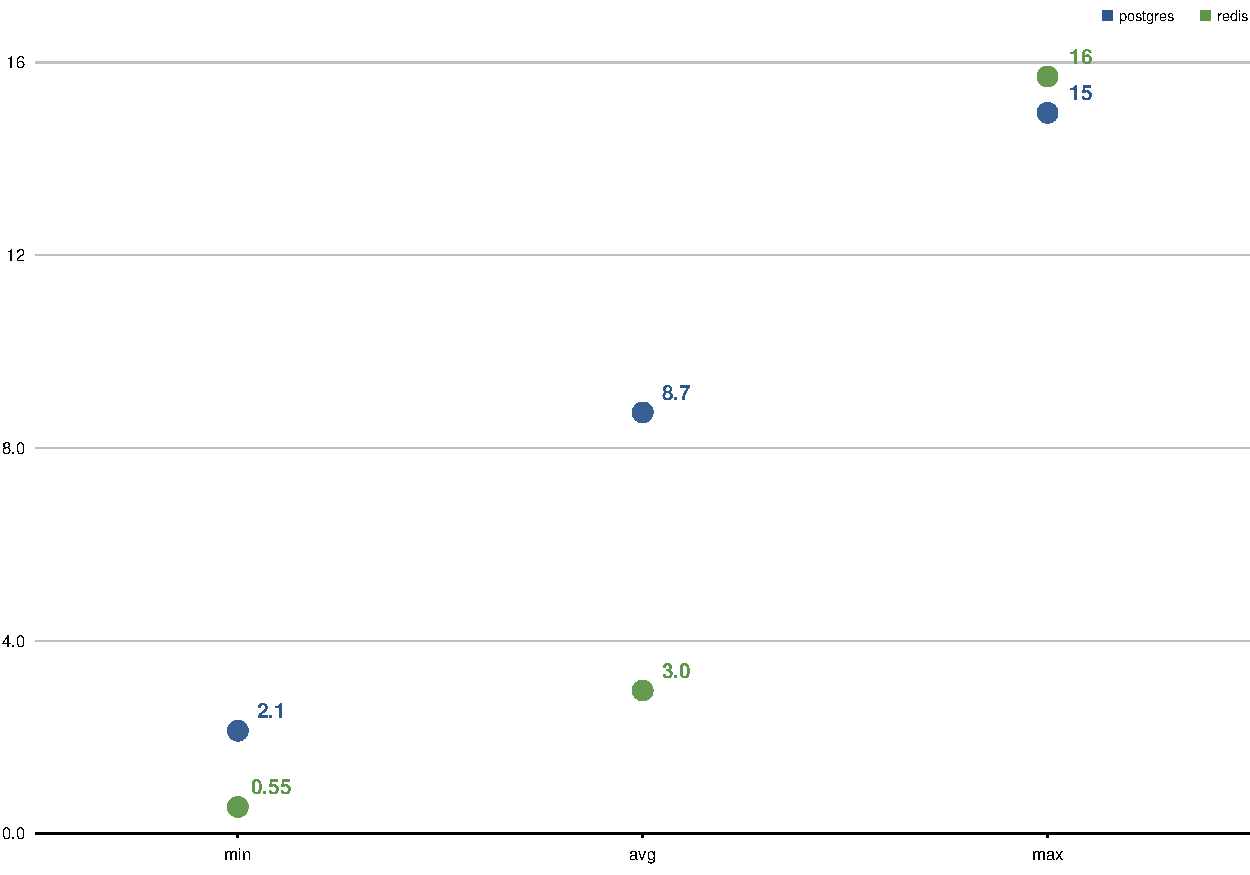
\includegraphics[width=\textwidth]{charts/1-1-1-min-avg-max}
    \caption{Minimalny, średni i maksymalny czas (w milisekundach, średnia z 5 uruchomień).}
  \end{subfigure}
  \begin{subfigure}{\textwidth}
    \centering
    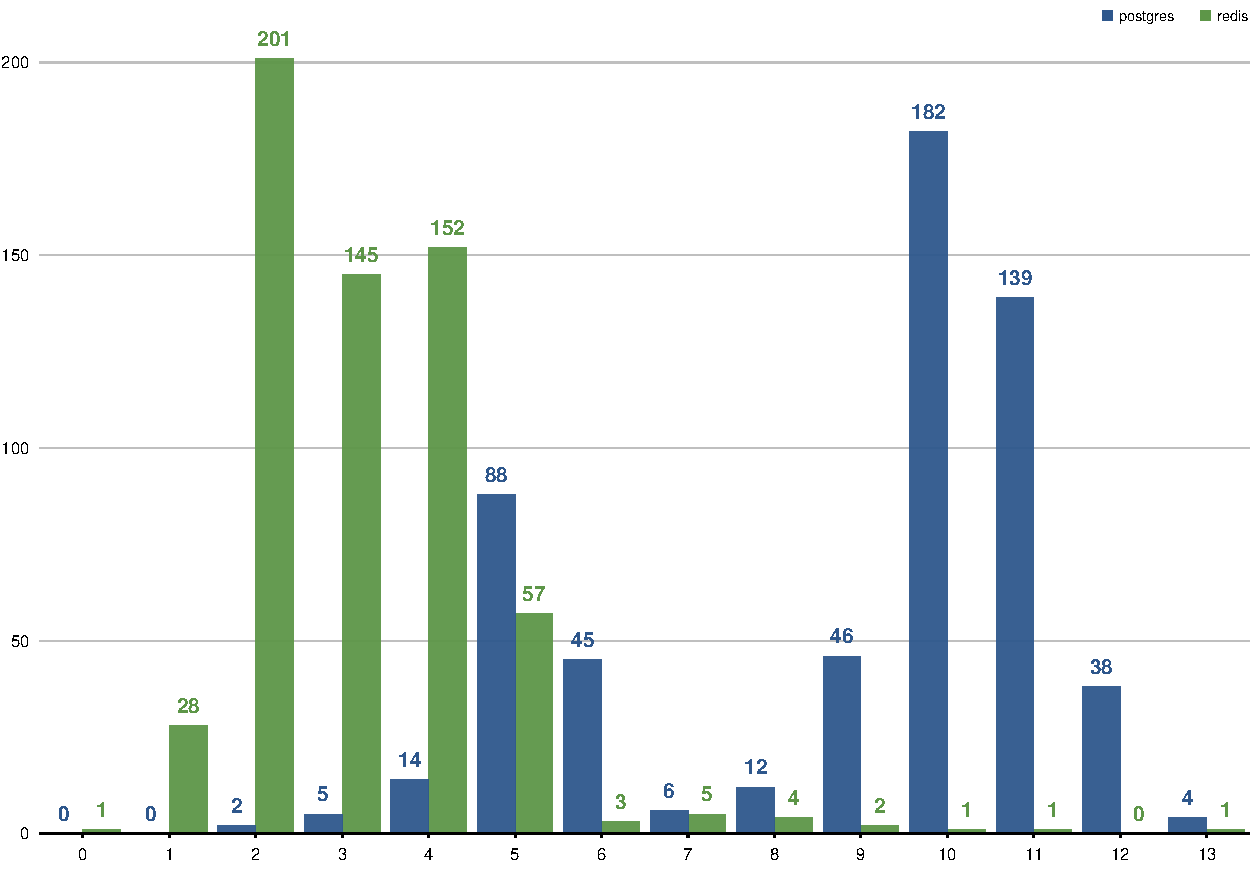
\includegraphics[width=\textwidth]{charts/1-1-1-grouped}
    \caption{Częstość wystąpień czasów w~zaokrągleniu do milisekundy (w ostatnim uruchomieniu).}
  \end{subfigure}
  \caption{Po jednym procesie każdego typu, 1500 requestów.}
  \label{1-1-1}
\end{figure}


\subsection{Po dwa procesy każdego typu, 3000 requestów}

Dwa procesy typu 1 zgłaszają po 1500 żądań (czyli łącznie jest 3000 requestów), przetwarzają je po dwa procesy typu 2 i typu 3 (rysunek \ref{2-2-2}).
\begin{figure}[h!]
  \centering
  \begin{subfigure}{\textwidth}
    \centering
    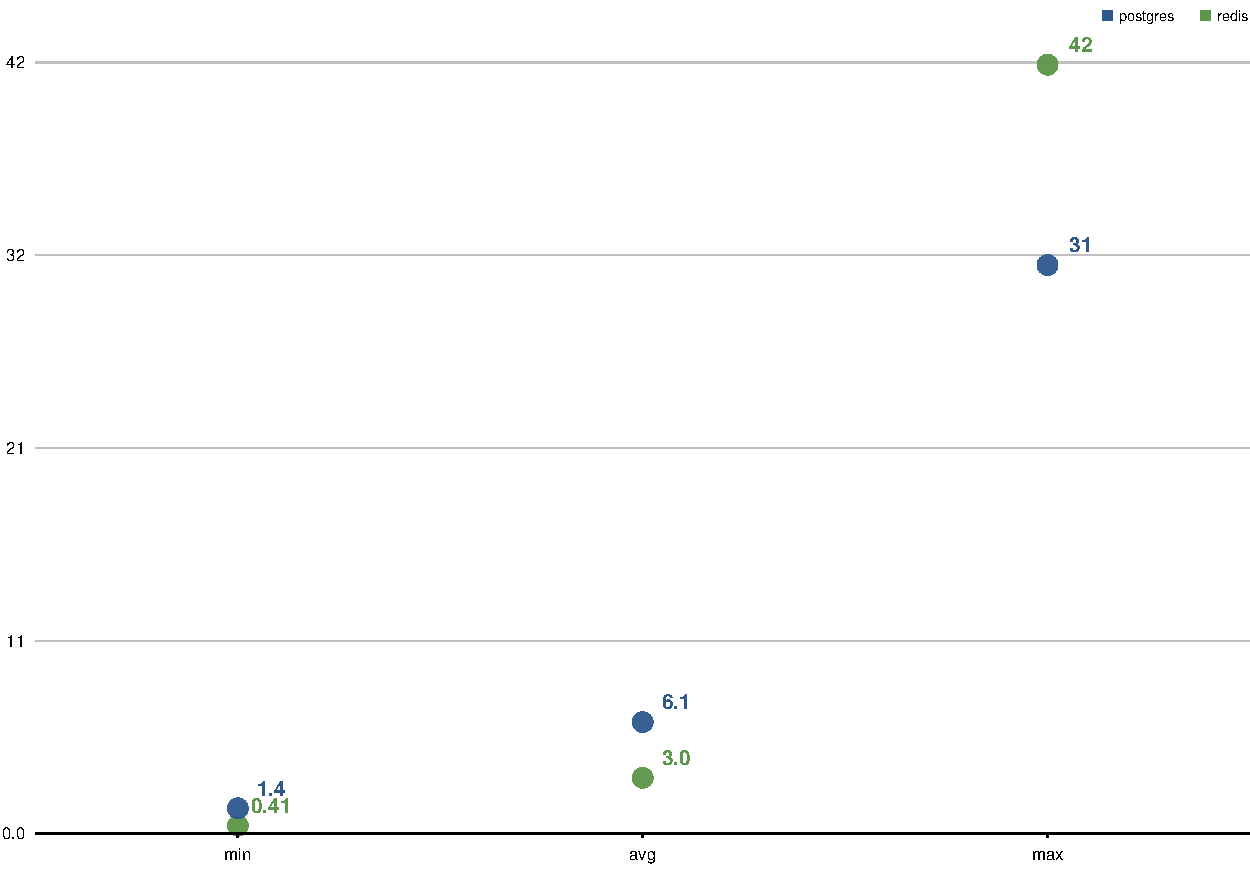
\includegraphics[width=\textwidth]{charts/2-2-2-min-avg-max}
    \caption{Minimalny, średni i maksymalny czas (w milisekundach, średnia z 5 uruchomień).}
  \end{subfigure}
  \begin{subfigure}{\textwidth}
    \centering
    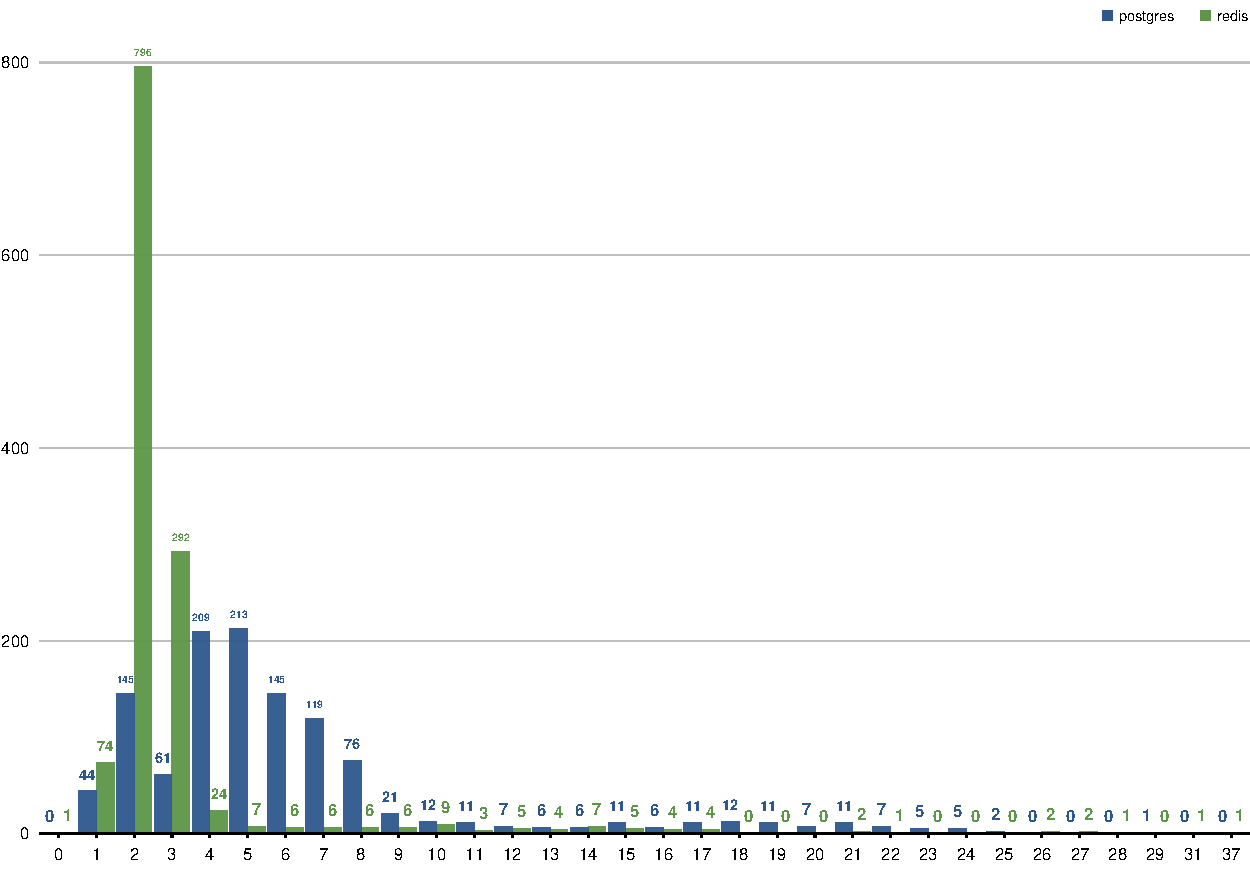
\includegraphics[width=\textwidth]{charts/2-2-2-grouped}
    \caption{Częstość wystąpień czasów w~zaokrągleniu do milisekundy (w ostatnim uruchomieniu).}
  \end{subfigure}
  \caption{Po dwa procesy każdego typu, 3000 requestów.}
  \label{2-2-2}
\end{figure}


\subsection{Po cztery procesy każdego typu, 6000 requestów}

Cztery procesy typu 1 zgłaszają po 1500 żądań (czyli łącznie jest 6000 requestów), przetwarzają je po cztery procesy typu 2 i typu 3 (rysunek \ref{4-4-4}).
\begin{figure}[h!]
  \centering
  \begin{subfigure}{\textwidth}
    \centering
    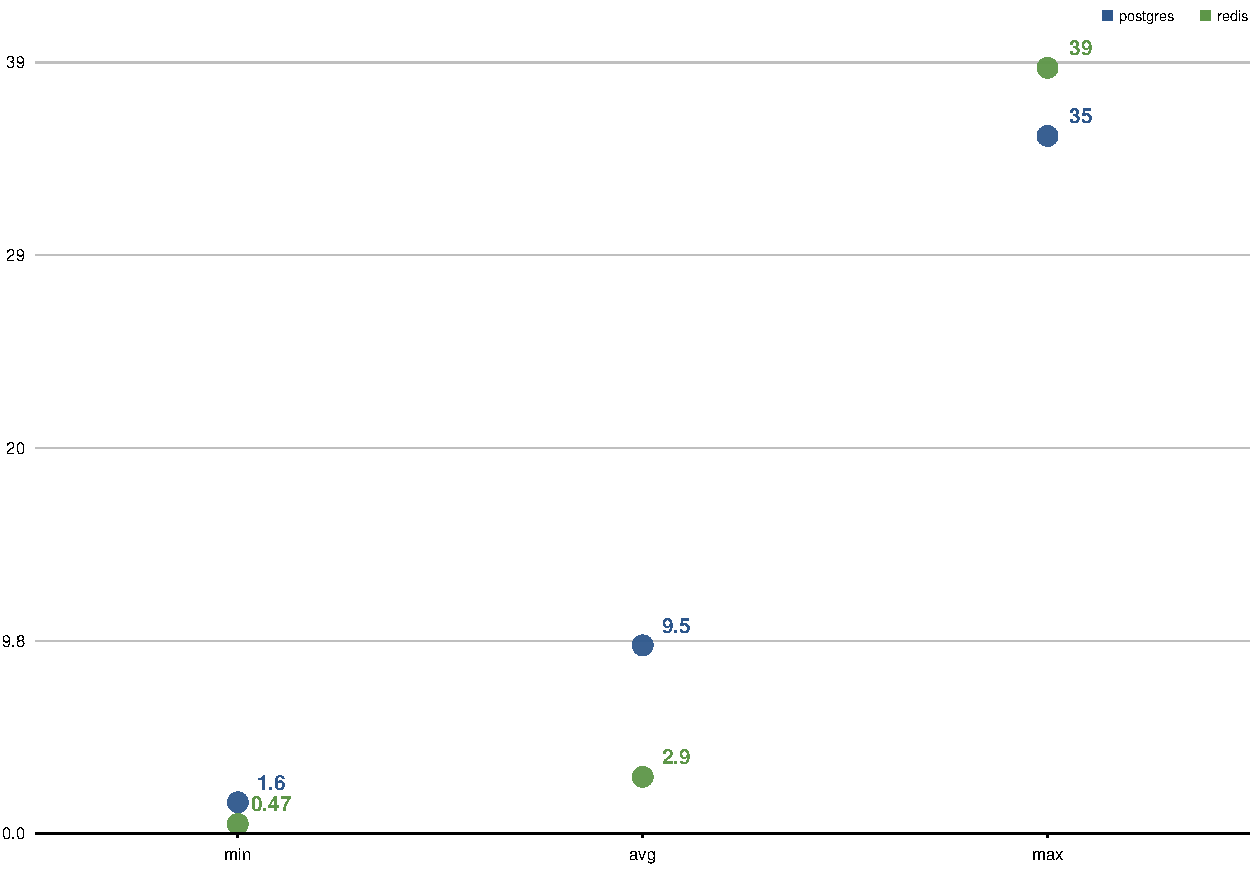
\includegraphics[width=\textwidth]{charts/4-4-4-min-avg-max}
    \caption{Minimalny, średni i maksymalny czas (w milisekundach, średnia z 5 uruchomień).}
  \end{subfigure}
  \begin{subfigure}{\textwidth}
    \centering
    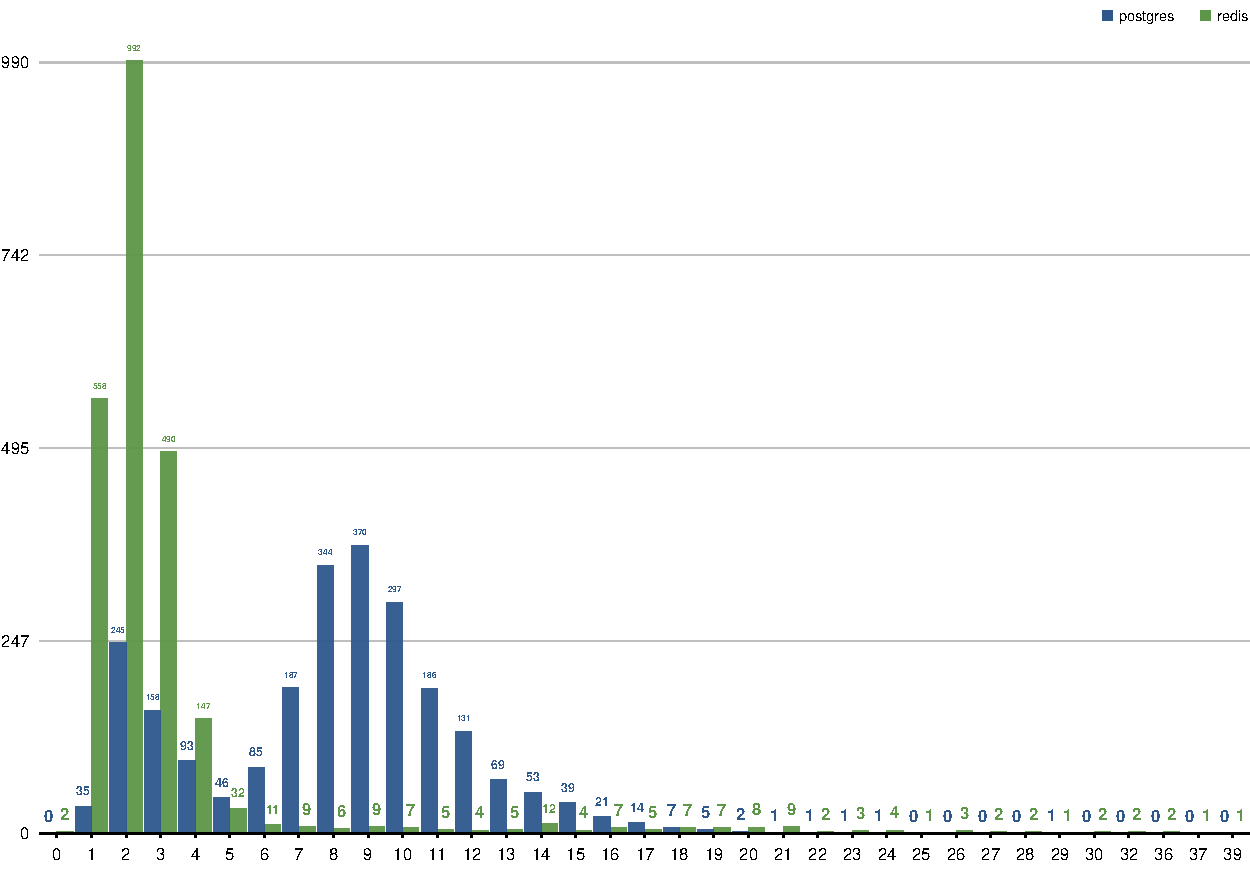
\includegraphics[width=\textwidth]{charts/4-4-4-grouped}
    \caption{Częstość wystąpień czasów w~zaokrągleniu do milisekundy (w ostatnim uruchomieniu).}
  \end{subfigure}
  \caption{Po cztery procesy każdego typu, 6000 requestów.}
  \label{4-4-4}
\end{figure}


\subsection{Jeden proces typu 1, po dwa procesy typu 2 i 3, 1500 requestów}

Jeden proces typu 1 zgłasza 1500 żądań, przetwarzają je po dwa procesy typu 2 i typu 3 (rysunek \ref{1-2-2}).
\begin{figure}[h!]
  \centering
  \begin{subfigure}{\textwidth}
    \centering
    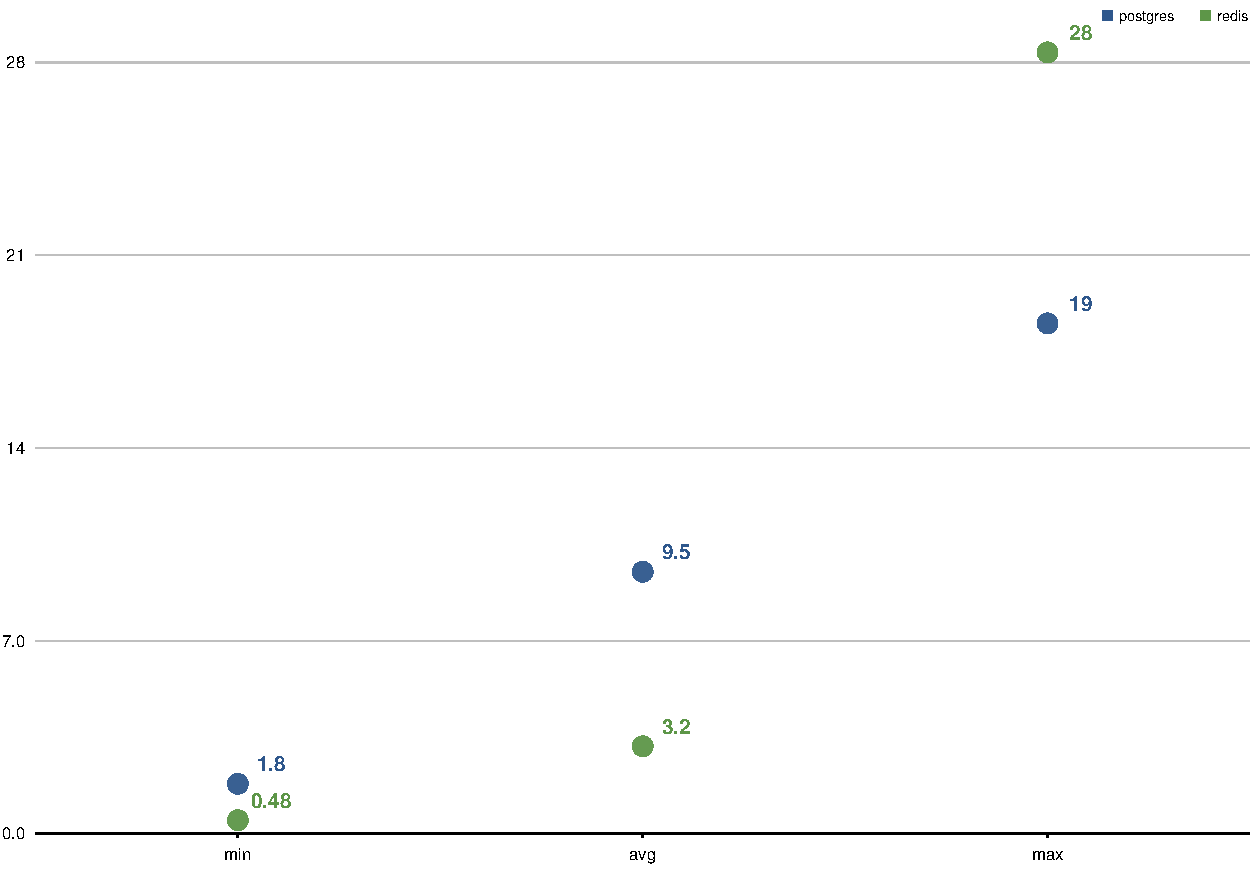
\includegraphics[width=\textwidth]{charts/1-2-2-min-avg-max}
    \caption{Minimalny, średni i maksymalny czas (w milisekundach, średnia z 5 uruchomień).}
  \end{subfigure}
  \begin{subfigure}{\textwidth}
    \centering
    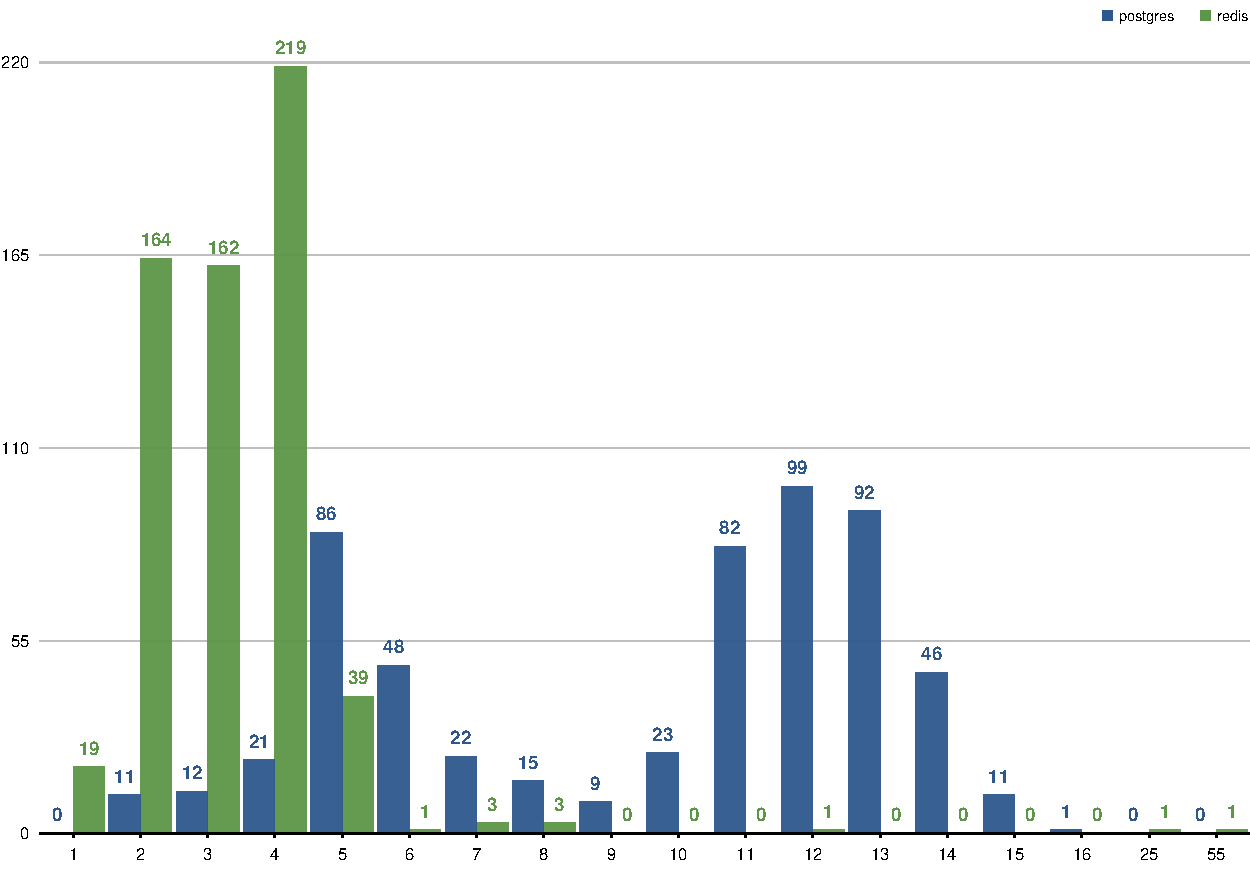
\includegraphics[width=\textwidth]{charts/1-2-2-grouped}
    \caption{Częstość wystąpień czasów w~zaokrągleniu do milisekundy (w ostatnim uruchomieniu).}
  \end{subfigure}
  \caption{Jeden proces typu 1, po dwa procesy typu 2 i 3, 1500 requestów.}
  \label{1-2-2}
\end{figure}


\section{Podsumowanie}

Minimalne i średnie czasy potrzebne na emisję reklamy za każdym razem są zdecydowanie mniejsze w wersji opartej na redisie.
Maksymalne czasy są mniejsze w wersji opartej na postgresie, ale w~każdej sytuacji decydują o tym pojedyncze przypadki
z wersji redis. Potwierdzają to wykresy częstości wystąpień czasów w~zaokrągleniu do milisekundy --- najwięcej przypadków
w wersji redis osiąga czas poniżej 5 milisekund. Za to w wersji postgres często występują czasy około 10 milisekund.


\end{document}
